\section{Rationaler autonomer Agent als Probleml�ser}

Ein rationaler autonomer Agent ist ein Wesen, das seine Welt permanent wahrnehmen und unabh�ngig reagieren kann.

\begin{figure}[H]
    \centering
    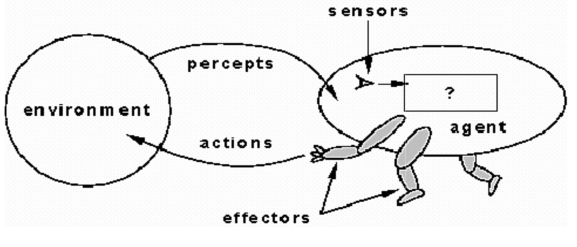
\includegraphics[width=0.8\textwidth]{figures/rational-agent.png}
    \caption{Rationaler autonomer Agent}
    \label{fig:rational-agent-diagram}
\end{figure}

Die Abbildung \ref{fig:rational-agent-diagram} veranschaulicht die Interaktion zwischen einem Agenten und seiner Umgebung unter Verwendung seiner Perzeptoren (PAGE = Percepts, Actions, Goals, Environment). 

\subsection{Vertiefung: Einfaches Beispiel f�r einen rationalen autonomen Agenten}

\begin{figure}[H]
    \centering
    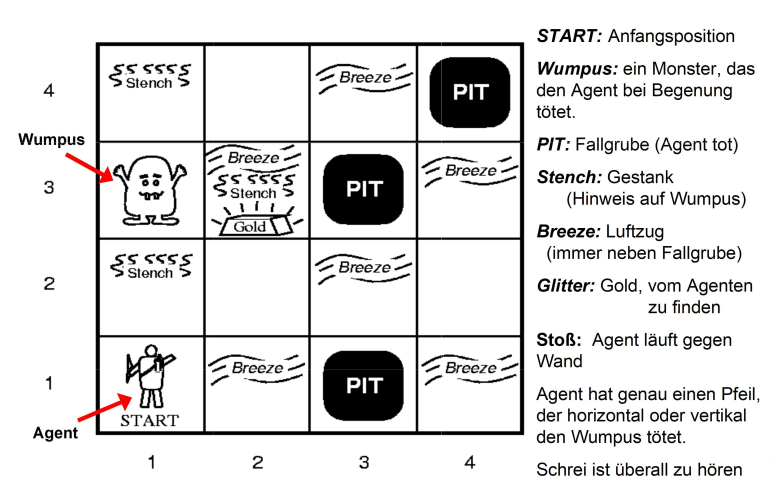
\includegraphics[width=0.8\textwidth]{figures/wumpus.png}
    \caption{Wumpus World}
    \label{fig:wumpus-example}
\end{figure}

Wumpus World ist eine H�hle mit 4/4 R�umen, die durch G�ngen verbunden sind. Es sind also insgesamt 16 R�ume miteinander verbunden. Es gibt einen wissensbasierten Agenten, der durch diese Welt gehen wird. Die H�hle hat einen Raum mit einem Monster namens Wumpus, das jeden frisst, der den Raum betritt. Wumpus kann vom Agenten erschossen werden, aber der Agent hat einen einzigen Pfeil. In der Welt von Wumpus gibt es mehrere endlose Lochr�ume und wenn ein Agent in ein Loch f�llt, wird er dort f�r immer gefangen sein. In einem der R�ume dieser H�hle befindet sich ein Haufen Gold. Das Ziel des Agenten ist es also, das Gold zu finden und aus der H�hle zu kommen, ohne in das Loch zu fallen oder von Wumpus gefressen zu werden. Der Agent wird belohnt, wenn er mit Gold herauskommt, und er bekommt eine Strafe, wenn er von Wumpus gefressen wird oder in ein Loch f�llt.

\paragraph{Umgebung von Wumpus World}
\begin{itemize}
    \item Ein 4x4-Raster von R�umen.
    \item Der Agent beginnt im Feld [1,1] und zeigt nach rechts.
    \item Standort von Wumpus und Gold werden zuf�llig ausgew�hlt, au�er Feld [1,1].
    \item Jedes Quadrat der H�hle kann mit Wahrscheinlichkeit 0,2 eine Grube sein, au�er dem ersten Quadrat
\end{itemize}

\paragraph{Eigenschaften von Wumpus World}
\begin{itemize}
    \item Die Welt ist teilweise beobachtbar, da der Agent nur die nahe Umgebung wahrnehmen kann, in der er sich befindet.
    \item Die Welt ist deterministisch, da die Auswirkungen aller Handlungen bekannt sind.
    \item Die Reihenfolge ist wichtig, also ist die Welt sequentiell.
    \item Die Welt ist statisch wie Wumpus und die Gruben bewegen sich nicht.
    \item Die Umgebung ist diskret.
    \item Einzelagentenumgebung (Wumpus wird nicht als Agent betrachtet, da er statisch ist).
\end{itemize}

\subsection{Arten von rationalen Agenten}

\paragraph{Reflex Agenten}

Ein Reflexagent ist eine Entit�t, die reaktiv ist und mit Sensoren arbeitet. Dieser Agent setzt sich keine Ziele und k�mmert sich nicht um die Auswirkungen seiner Handlungen.

\begin{figure}[H]
    \centering
    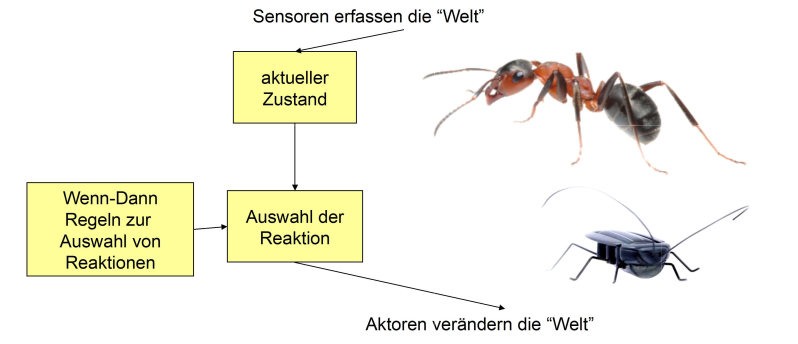
\includegraphics[width=0.8\textwidth]{figures/reflex-agent.png}
    \caption{Reflex-Agenten}
    \label{fig:reflex-agent}
\end{figure}

\paragraph{Ziel orientierter Agent}

Zielorientierte Agenten planen ihre Handlungen und antizipieren die Auswirkungen dieser Handlungen, um ihre Ziele zu erreichen.

\begin{figure}[H]
    \centering
    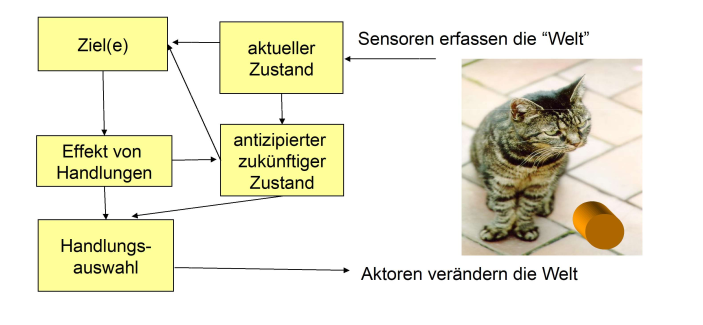
\includegraphics[width=0.8\textwidth]{figures/goal-oriented-agents.png}
    \caption{Ziel-orientierter Agenten}
    \label{fig:ziel-orientierter-agent}
\end{figure}

\newpage
\paragraph{Nutzen-orientierter Agent}

Ein nutzen-orientierter Agent w?gt die Kosten und Gewinne von Handlungen ab, um die Effektivit�t seiner Handlungen beim Erreichen eines Ziels zu maximieren.

\begin{figure}[H]
    \centering
    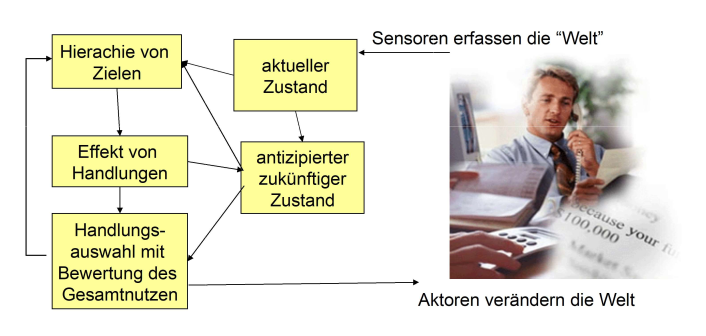
\includegraphics[width=0.6\textwidth]{figures/nutzen-orientierter-agent.png}
    \caption{Nutzen-orientierter Agenten}
    \label{fig:nutzen-orientierter-agent}
\end{figure}

\paragraph{Lern-f?higer Agent}

Diese Art von Agent ist in der Lage, die Effekte seiner Handlungen zu lernen, um seine Ziele besser zu erreichen, indem er seine Handlungen effektiver ausw�hlt.

\begin{figure}[H]
    \centering
    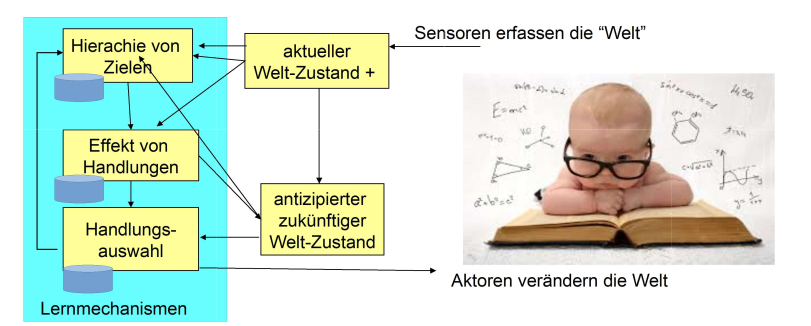
\includegraphics[width=0.8\textwidth]{figures/lern-agent.png}
    \caption{Lern-f�higer Agenten}
    \label{fig:lernen-agent}
\end{figure}

\paragraph{Emotionaler Agent}

Dieser Agent verwendet neben rationalem Denken eine emotionale Bewertung, um reale menschliche Entscheidungsprozesse besser zu simulieren.

\begin{figure}[H]
    \centering
    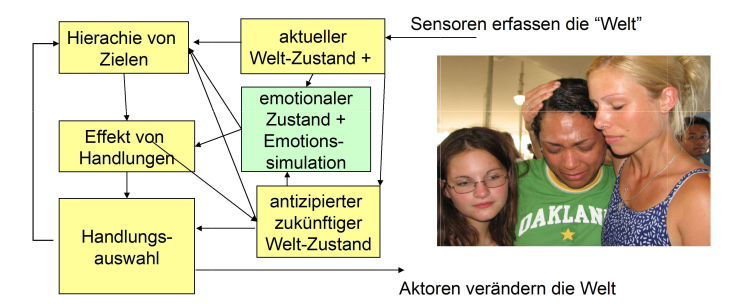
\includegraphics[width=0.8\textwidth]{figures/emotionaler-agent.png}
    \caption{Emotionaler Agent}
    \label{fig:emo-agent}
\end{figure}

\paragraph{Kreativer Agent}

Dieser Agent hat die F�higkeit, neue Aktionen zu entwickeln, um neue Wege zur L�sung von Problemen zu schaffen, die nicht vorprogrammiert waren.

\begin{figure}[H]
    \centering
    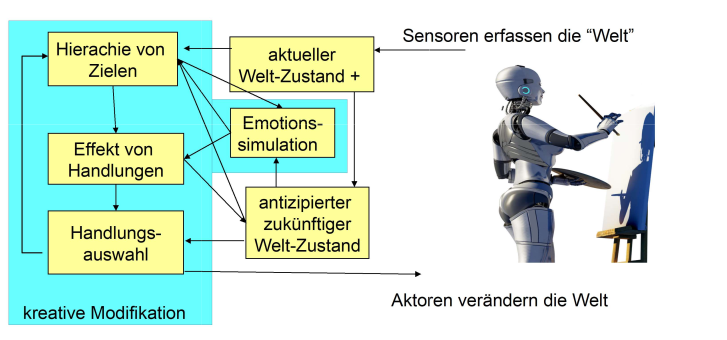
\includegraphics[width=0.8\textwidth]{figures/creative-agent.png}
    \caption{Kreativer Agent}
    \label{fig:creative-agent}
\end{figure}


\paragraph{Kooperative Agenten}

Eine Situation, in der mehrere Agenten zusammenarbeiten, um komplexe Aufgaben zu l�sen. Dies erfordert die Modellierung kooperativer Verhaltensstrategien und das Verst�ndnis der Absichten anderer Agenten.

\begin{figure}[H]
    \centering
    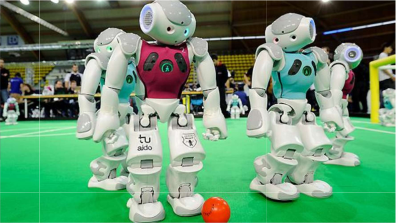
\includegraphics[width=0.8\textwidth]{figures/robocup.png}
    \caption{Robocup competition: Cooperative agents}
    \label{fig:coop-agent}
\end{figure}

Mit PDDL kann man Cloud-basierte Planungsdienste nutzen. Es gibt Implementierungen von Hochleistungsplanern, die als Cloud-Dienste verf�gbar sind, wobei die Planungsaufgabe und -dom�ne in PDDL definiert und das Ergebnis ?ber eine API abgerufen wird.